%************************************************
\chapter{Introducción}\label{ch:introduccion}
% ************************************************

\noindent La mecánica cuántica es un área de la física que describe sistemas a escalas atómicas. Su entendimiento fue cuestionado por las personas de la época en sus inicios (1920's), pues sus fundamentos eran ideas revolucionarias y contra intuitivas comparadas con la descripción de la naturaleza que ofrecía la mecánica que hasta entonces se conocía: la mecánica clásica, pues con la información suficiente de un sistema físico, esta ofrecía respuestas concretas al predecir su evolución en el tiempo. La mecánica cuántica por otro lado, plantea sus respuestas en términos de una densidad de probabilidad, en donde, hasta hacer una medición, se puede saber con exactitud la variable física del sistema que se quiere estudiar. La interpretación de la mecánica cuántica sigue siendo un tema que genera discusión, sin embargo, la validez y fortaleza de la teoría no son puestas en duda, pues es capaz de explicar el comportamiento y las interacciones de las partículas a pequeña escala de manera exitosa y de acuerdo a las pruebas experimentales.
\\

La evolución temporal de un sistema cuántico es de gran interés para diferentes áreas de la ciencia, pues tiene diversas aplicaciones en procesos químicos y biológicos. En tales procesos es importante tener una descripción cuántica del sistema, ya que trata de interacciones a niveles atómicos o moleculares. La ecuación de Schrödinger dependiente del tiempo, (\acs{TDSE}, por sus siglas en inglés), es la ecuación que describe la evolución temporal de un sistema cuántico; por otro lado, el Hamiltoniano de un sistema, en el formalismo de la mecánica cuántica, es un operador que contiene la información de la energía total del sistema.
\\
El Hamiltoniano caracteriza las interacciones en un sistema físico, por lo tanto, la solución a la ecuación de Schrödinger depende del Hamiltoniano. Muchos procesos químicos implican una dependencia temporal, lo que conduce a un Hamiltoniano complejo. Para resolver la \acs{TDSE} y encontrar una descripción de la evolución del sistema, se pueden emplear diversos métodos analíticos o numéricos; sin embargo, dependiendo de la naturaleza del sistema, los cálculos o su tiempo de cómputo pueden llegar a representar un problema para obtener resultados de manera eficiente.
\\
\\
En los últimos años, las redes neuronales artificiales (\acs{ANN}s, por sus siglas en inglés) han sido modelos de aprendizaje automático que han cobrado popularidad debido a los avances en computación, al uso de unidades de procesamiento gráfico (GPU's, por sus siglas en inglés), al mejoramiento en algoritmos y modelos; y al incremento de datos. Actualmente pueden ofrecer resultados que consumen menos tiempo y/o memoria de cómputo en diversos problemas con una precisión exitosa. De la manera más general, las \acs{ANN}s pueden verse como modelos computacionales, cuya forma de aprender\footnote{Históricamente las \acs{ANN}s fueron inspiradas por las estructuras neuronales biológicas; un concepto como el \emph{entrenamiento} de una \acs{ANN}, puede interpretarse como el proceso análogo de \emph{aprendizaje} que tienen los organismos biológicos.} se basa en procesar ejemplos de datos referentes al problema o sistema en cuestión.
\\
\\
El objetivo de este trabajo es implementar una \acs{ANN} que funcione como propagador para cierto tipo de sistemas cuánticos dependientes del tiempo. Es decir, una \acs{ANN} que mapee en un periodo largo de tiempo $\{t_0,t_1,\cdots t_n\}$ una función de onda en un tiempo inicial $\psi(r,t)$ a un intervalo de tiempo posterior $\psi(r,t+\Delta t)$ bajo potenciales que dependen del tiempo, obteniendo así un modelo alternativo a los métodos analíticos y numéricos para la resolución de la \acs{TDSE} para este tipo de sistemas.

\section{Organización}

\noindent En la segunda parte de la tesis (\autoref{pt:TDSE}) se abordan los conceptos básicos de dinámica cuántica y la ecuación de Schrödinger dependiente del tiempo para la descripción de la evolución temporal de sistemas cuánticos. En el \autoref{ch:DVR} se desarrolla un ejemplo de método numérico para la resolución de la \acs{TDSE} aplicada al tipo de sistemas cuánticos de interés para este trabajo.\\

La tercera parte de la tesis (\autoref{pt:ANNS}) describe una breve introducción sobre aprendizaje automático y aprendizaje supervisado, posteriormente se describen los fundamentos y características principales de las redes neuronales artificiales (\acs{ANN}s).\\


La última parte de la tesis (\autoref{pt:Modelos}) comienza describiendo las redes neuronales recurrentes, (\acs{RNN}s, por sus siglas en inglés), un tipo de redes neuronales artificiales que es útil para abordar sistemas descritos en secuencias de tiempo.\\
En la sección 6.4 se implementa una red neuronal recurrente para predecir la evolución de un paquete de onda bajo un potencial dependiente del tiempo característico de los sistemas de transferencia de protones (\autoref{sec:ProtonTransfer}). En las secciones \autoref{sec:6.4.1} y \autoref{sec:6.4.2} se desarrollan los métodos computacionales utilizados para la generación y procesamiento de los datos de entrenamiento, en la sección \autoref{sec:6.4.3} se describen los detalles de la red neuronal artificial relacionados con su arquitectura y entrenamiento, en la sección \autoref{sec:Resultados} se muestra la precisión del modelo y sus predicciones. Finalmente, en el \autoref{ch:Conclusiones} se presentan las conclusiones del trabajo, así como sugerencias para implementar en proyectos futuros relacionados.



%\begin{marginfigure}%
 % \caption{\emph{Caracol}. Yucatán, México. Proto-observatorio.}
  %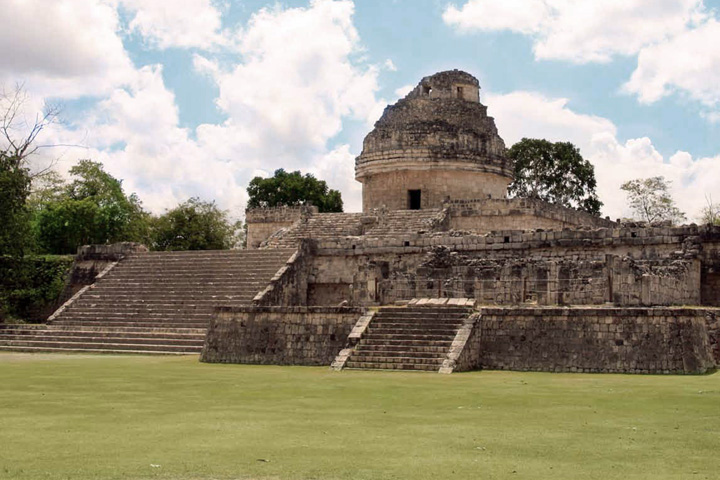
\includegraphics[width=\marginparwidth]{figures/caracol.jpg}
 % \label{fig:caracol}
%\end{marginfigure}





